% Provenance (never printed): see sources/outline_sources.md and sources/book1/BRIEFS.md (g8/01).
\chapter{Binary and Hexadecimal}\label{ch:g8:binary-and-hexadecimal}

The \omterm{def:g5:networks-first-look:page}{web page} of Noor's football club writes its orange as \texttt{\#FF8800}. A
colour, written with letters? The letters are digits: \code{FF8800} is a
number, written in base 16. This chapter explains how numbers are written in
base 2, the base of the machine, and in base 16, the short way people write
base 2.

\begin{recall}
A \omterm{def:g5:bits-and-bytes:bit}{bit} is a 0 or a 1, a \omterm{def:g4:memory-and-storage:byte}{byte} is eight \omterm{def:g5:bits-and-bytes:bit}{bits}, and each extra \omterm{def:g5:bits-and-bytes:bit}{bit} doubles the
number of patterns (\cref{ch:g5:bits-and-bytes}). A colour on a screen is
made of three numbers from 0 to 255, for red, green and blue
(\cref{ch:g5:text-pictures-sound-as-numbers}). In mathematics, the place of a
digit gives its \omterm{def:g6:variables-and-input:value}{value} (in 352, the 3 is worth 300), and $2^5$ means
$2 \times 2 \times 2 \times 2 \times 2$.
\end{recall}

\section{Place value in base 2}

\begin{definition}[Number base]\label{def:g8:binary-and-hexadecimal:base}
A \emph{number base}\index{number base} is the number of digits a way of
writing numbers uses. In base $b$, each place is worth $b$ times the place on
its right: the places are worth 1, $b$, $b^2$, $b^3$, and so on, from the
right.
\end{definition}

Our usual numbers are in base 10: the places are worth 1, 10, 100, 1\,000.
\omterm{def:g5:bits-and-bytes:binary}{Binary} is base 2: the places are worth 1, 2, 4, 8, 16, 32\dots, the powers of
2, exactly the dots on the cards of \cref{ch:g5:bits-and-bytes}. A \omterm{def:g5:bits-and-bytes:binary}{binary
number} is the sum of the places where it has a 1.

\begin{omfigure}
\begin{tikzpicture}[x=1cm, y=1cm, font=\footnotesize]
  \foreach \p/\d [count=\i from 0] in {1000/0, 100/3, 10/5, 1/2} {
    \draw[black!60, fill=ocBlue!10] (1.3*\i,0.6) rectangle ++(1.3,0.5);
    \node at (1.3*\i+0.65,0.85) {\p};
    \draw[black!60, fill=ocYellow!20] (1.3*\i,0) rectangle ++(1.3,0.6);
    \node[font=\small] at (1.3*\i+0.65,0.3) {\d};
  }
  \node[anchor=west] at (0,-0.35) {$3 \times 100 + 5 \times 10 + 2 = 352$};
  \foreach \p/\d [count=\i from 0] in {32/1, 16/0, 8/1, 4/1, 2/0, 1/0} {
    \draw[black!60, fill=ocBlue!10] (6.2+0.9*\i,0.6) rectangle ++(0.9,0.5);
    \node at (6.2+0.9*\i+0.45,0.85) {\p};
    \draw[black!60, fill=ocYellow!20] (6.2+0.9*\i,0) rectangle ++(0.9,0.6);
    \node[font=\small] at (6.2+0.9*\i+0.45,0.3) {\d};
  }
  \node[anchor=west] at (6.2,-0.35) {$32 + 8 + 4 = 44$};
  \node[font=\bfseries] at (2.6,1.45) {base 10};
  \node[font=\bfseries] at (8.9,1.45) {base 2};
\end{tikzpicture}

{\small The same idea in two bases: the \omterm{def:g6:variables-and-input:value}{value} of each place, and the digits of
352 in base 10 and of 44 in base 2.}
\end{omfigure}

To read a \omterm{def:g5:bits-and-bytes:binary}{binary number} with a \omterm{def:g4:programs-and-operating-system:program}{program}, walk through its \omterm{def:g5:bits-and-bytes:bit}{bits} from the left.
Each new \omterm{def:g5:bits-and-bytes:bit}{bit} shifts everything one place to the left, which doubles the \omterm{def:g6:variables-and-input:value}{value}
so far, then adds itself.

\Needspace*{9\baselineskip}
\omcode{code/grade-8/01-binary-and-hexadecimal/listings/to_decimal.py}{1}{6}{From
\omterm{def:g5:bits-and-bytes:binary}{binary} to decimal.}\label{lst:g8:binary-and-hexadecimal:to-decimal}

\Needspace*{11\baselineskip}
\omoutput{code/grade-8/01-binary-and-hexadecimal/outputs/to_decimal.txt}{The \omterm{def:g6:variables-and-input:value}{value}
after each \omterm{def:g5:bits-and-bytes:bit}{bit}.}\label{out:g8:binary-and-hexadecimal:to-decimal}

\section{Converting both ways}

The other way, from decimal to \omterm{def:g5:bits-and-bytes:binary}{binary}, divides by 2 again and again. The
remainder of each division, 0 or 1, is the next \omterm{def:g5:bits-and-bytes:bit}{bit} from the right, and the
quotient is what remains to be written.

\begin{method}[Decimal to binary]\label{met:g8:binary-and-hexadecimal:division}
Divide the number by 2, and write down the remainder. Divide the quotient by 2
again, and go on until the quotient is 0. The remainders, read from the last
to the first, are the \omterm{def:g5:bits-and-bytes:bit}{bits} of the number.
\end{method}

\begin{omfigure}
\begin{tikzpicture}[x=1cm, y=0.55cm, font=\footnotesize]
  \foreach \n/\q/\r [count=\i from 0] in {44/22/0, 22/11/0, 11/5/1, 5/2/1, 2/1/0, 1/0/1} {
    \node[anchor=east] at (1.2,-\i) {$\n \div 2 =$};
    \node[anchor=west] at (1.3,-\i) {$\q$, remainder};
    \node[draw=black!60, fill=ocYellow!25, minimum width=0.5cm, minimum height=0.45cm] at (3.7,-\i) {\r};
  }
  \draw[-{Stealth[length=2mm]}, very thick, ocRed] (4.4,-5.2) -- node[right, align=left] {read upwards:\\ 101100} (4.4,0.2);
\end{tikzpicture}

{\small The division ladder for 44: the last remainder is the first \omterm{def:g5:bits-and-bytes:bit}{bit}.}
\end{omfigure}

\omcode{code/grade-8/01-binary-and-hexadecimal/listings/to_binary.py}{1}{11}{From
decimal to \omterm{def:g5:bits-and-bytes:binary}{binary}.}\label{lst:g8:binary-and-hexadecimal:to-binary}

\Needspace*{11\baselineskip}
\omoutput{code/grade-8/01-binary-and-hexadecimal/outputs/to_binary.txt}{Each
division, then the \omterm{def:g5:bits-and-bytes:bit}{bits}.}\label{out:g8:binary-and-hexadecimal:to-binary}

Python can check both \omterm{def:g4:programs-and-operating-system:program}{programs}. \code{bin} writes a number in \omterm{def:g5:bits-and-bytes:binary}{binary}, with
\code{0b} in front to show the base; \code{int(text, 2)} reads a text as a
\omterm{def:g5:bits-and-bytes:binary}{binary number}. A number can also be typed directly in \omterm{def:g5:bits-and-bytes:binary}{binary},
\code{0b101100}.

\Needspace*{6\baselineskip}
\omcode{code/grade-8/01-binary-and-hexadecimal/listings/base_functions.py}{1}{3}{Python's
own conversions.}\label{lst:g8:binary-and-hexadecimal:base-functions}

\Needspace*{7\baselineskip}
\omoutput{code/grade-8/01-binary-and-hexadecimal/outputs/base_functions.txt}{The
same 44, four times; \code{hex} and base 16 come in a few
pages.}\label{out:g8:binary-and-hexadecimal:base-functions}

\section{Adding in binary}

\omterm{def:g5:bits-and-bytes:binary}{Binary numbers} are added like decimal ones, column by column from the right,
but a column overflows as soon as it reaches 2: $1 + 1$ is 10 in \omterm{def:g5:bits-and-bytes:binary}{binary}, so
the column gets a 0 and a 1 goes into the next one.

\begin{definition}[Carry]\label{def:g8:binary-and-hexadecimal:carry}
In a column addition, the \emph{carry}\index{carry (in binary addition)} is
the digit passed to the next column on the left when a column's sum does not
fit in one digit. In \omterm{def:g5:bits-and-bytes:binary}{binary}, a column of $1 + 1$ writes 0 with a carry of 1,
and $1 + 1 + 1$ writes 1 with a carry of 1.
\end{definition}

\begin{omfigure}
\begin{tikzpicture}[x=0.6cm, y=0.6cm, font=\small\ttfamily]
  \foreach \c [count=\i from 0] in {1,1,1,1,1,1,1,} \node[ocRed, font=\scriptsize\ttfamily] at (\i+1,1.1) {\c};
  \foreach \d [count=\i from 0] in {0,1,1,0,1,1,0,1} \node at (\i+1,0) {\d};
  \foreach \d [count=\i from 0] in {0,0,1,1,1,0,1,1} \node at (\i+1,-1) {\d};
  \node at (-0.2,-1) {+};
  \draw (0.2,-1.6) -- (8.6,-1.6);
  \foreach \d [count=\i from 0] in {1,0,1,0,1,0,0,0} \node at (\i+1,-2.2) {\d};
  \node[font=\footnotesize\sffamily, anchor=west] at (9.2,0) {109};
  \node[font=\footnotesize\sffamily, anchor=west] at (9.2,-1) {59};
  \node[font=\footnotesize\sffamily, anchor=west] at (9.2,-2.2) {168};
  \node[font=\footnotesize\sffamily, anchor=west, ocRed] at (9.2,1.1) {carries};
\end{tikzpicture}

{\small Adding two \omterm{def:g4:memory-and-storage:byte}{bytes}: the carries, in red, ride above the columns.}
\end{omfigure}

The \omterm{def:g4:programs-and-operating-system:program}{program} does the same with two \omterm{def:g7:strings:string}{strings} of \omterm{def:g5:bits-and-bytes:bit}{bits}. It walks the columns from
the right with \code{range(len(a) - 1, -1, -1)}, which counts down to 0, and
keeps the \omterm{def:g8:binary-and-hexadecimal:carry}{carry} in a \omterm{def:g6:variables-and-input:value}{variable}:

\omcode{code/grade-8/01-binary-and-hexadecimal/listings/add_binary.py}{1}{15}{Column
addition of two \omterm{def:g7:strings:string}{strings} of \omterm{def:g5:bits-and-bytes:bit}{bits}.}\label{lst:g8:binary-and-hexadecimal:add}

\Needspace*{6\baselineskip}
\omoutput{code/grade-8/01-binary-and-hexadecimal/outputs/add_binary.txt}{$109 +
59 = 168$, then $200 + 112 = 312$, which needs nine
\omterm{def:g5:bits-and-bytes:bit}{bits}.}\label{out:g8:binary-and-hexadecimal:add}

The second sum has a \omterm{def:g8:binary-and-hexadecimal:carry}{carry} out of the leftmost column: the answer has nine
\omterm{def:g5:bits-and-bytes:bit}{bits} and no longer fits in a \omterm{def:g4:memory-and-storage:byte}{byte}. A machine that keeps only eight \omterm{def:g5:bits-and-bytes:bit}{bits} has
to do something about it; the next book explains what.

\section{Hexadecimal}

Long rows of 0s and 1s are hard to read and easy to mistype. People therefore
write them in base 16.

\begin{definition}[Hexadecimal]\label{def:g8:binary-and-hexadecimal:hexadecimal}
\emph{Hexadecimal}\index{hexadecimal} is base 16. Its sixteen
\emph{hexadecimal digits}\index{hexadecimal digit} are 0 to 9, then A, B, C,
D, E and F for ten to fifteen.
\end{definition}

Since $16 = 2^4$, one \omterm{def:g8:binary-and-hexadecimal:hexadecimal}{hexadecimal digit} stands for exactly four \omterm{def:g5:bits-and-bytes:bit}{bits}. To turn
\omterm{def:g5:bits-and-bytes:binary}{binary} into \omterm{def:g8:binary-and-hexadecimal:hexadecimal}{hexadecimal}, cut the \omterm{def:g5:bits-and-bytes:bit}{bits} into groups of four from the right, and
write each group as one digit:

\begin{omfigure}
\begin{tikzpicture}[x=0.65cm, y=1cm, font=\small\ttfamily]
  \foreach \d [count=\i from 0] in {1,0,1,0,1,0,0,0} {
    \ifnum\i<4 \def\shade{ocBlue!15}\else\def\shade{ocMint!30}\fi
    \draw[black!60, fill=\shade] (\i,0) rectangle ++(1,0.7);
    \node at (\i+0.5,0.35) {\d};
  }
  \draw[thick, decorate, decoration={brace, amplitude=4pt, mirror}] (0,-0.1) -- (4,-0.1) node[midway, below=5pt, font=\small\sffamily] {$8 + 2 = 10$: \texttt{A}};
  \draw[thick, decorate, decoration={brace, amplitude=4pt, mirror}] (4,-0.1) -- (8,-0.1) node[midway, below=5pt, font=\small\sffamily] {$8$: \texttt{8}};
  \node[font=\small\sffamily, anchor=west] at (8.5,0.35) {$= $ \texttt{A8} $= 10 \times 16 + 8 = 168$};
\end{tikzpicture}

{\small A \omterm{def:g4:memory-and-storage:byte}{byte} is two \omterm{def:g8:binary-and-hexadecimal:hexadecimal}{hexadecimal digits}: one for each group of four \omterm{def:g5:bits-and-bytes:bit}{bits}.}
\end{omfigure}

\omcode{code/grade-8/01-binary-and-hexadecimal/listings/to_hex.py}{1}{14}{\omterm{def:g5:bits-and-bytes:binary}{Binary}
to \omterm{def:g8:binary-and-hexadecimal:hexadecimal}{hexadecimal}, four \omterm{def:g5:bits-and-bytes:bit}{bits} at a time.}\label{lst:g8:binary-and-hexadecimal:to-hex}

\Needspace*{7\baselineskip}
\omoutput{code/grade-8/01-binary-and-hexadecimal/outputs/to_hex.txt}{Sixteen \omterm{def:g5:bits-and-bytes:bit}{bits}
are only four \omterm{def:g8:binary-and-hexadecimal:hexadecimal}{hexadecimal digits}.}\label{out:g8:binary-and-hexadecimal:to-hex}

In Python, \code{hex} writes a number in \omterm{def:g8:binary-and-hexadecimal:hexadecimal}{hexadecimal} with \code{0x} in front,
\code{int(text, 16)} reads one, and \code{0x2C} can be typed directly
(\cref{out:g8:binary-and-hexadecimal:base-functions}). Python writes the
letters in small type, \code{0xff}; both are correct.

\section{Colours, and what $n$ bits can hold}

% ledger: g8:css-hex-colour
A colour in a \omterm{def:g5:networks-first-look:page}{web page} is written \texttt{\#RRGGBB}: a \texttt{\#}, then three
pairs of \omterm{def:g8:binary-and-hexadecimal:hexadecimal}{hexadecimal digits}, for red, green and blue. Each pair is one \omterm{def:g4:memory-and-storage:byte}{byte},
from \code{00} to \code{FF}, that is from 0 to 255.

\Needspace*{13\baselineskip}
\omcode{code/grade-8/01-binary-and-hexadecimal/listings/colours.py}{1}{10}{Three
colours split into their three numbers.}\label{lst:g8:binary-and-hexadecimal:colours}

\Needspace*{7\baselineskip}
\omoutput{code/grade-8/01-binary-and-hexadecimal/outputs/colours.txt}{Red, green
and blue of each colour.}\label{out:g8:binary-and-hexadecimal:colours}

\begin{omfigure}
\definecolor{clubOrange}{HTML}{FF8800}
\definecolor{seaGreen}{HTML}{2E8B57}
\definecolor{royalBlue}{HTML}{4169E1}
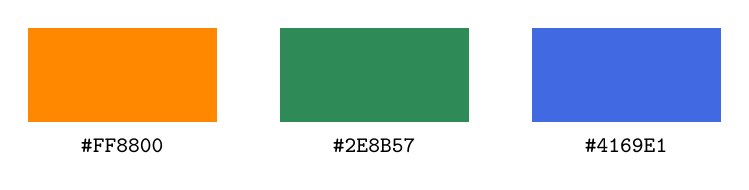
\begin{tikzpicture}[x=1cm, y=1cm, font=\footnotesize\ttfamily]
  \foreach \c/\t [count=\i from 0] in {clubOrange/\#FF8800, seaGreen/\#2E8B57, royalBlue/\#4169E1} {
    \fill[\c] (3.2*\i,0) rectangle ++(2.4,1.2);
    \node at (3.2*\i+1.2,-0.3) {\t};
  }
\end{tikzpicture}

{\small The three colours of \cref{lst:g8:binary-and-hexadecimal:colours},
drawn from the same codes.}
\end{omfigure}

Why do the three numbers stop at 255? Because a \omterm{def:g4:memory-and-storage:byte}{byte} has 8 \omterm{def:g5:bits-and-bytes:bit}{bits}, and 8 \omterm{def:g5:bits-and-bytes:bit}{bits}
make 256 patterns. The doubling of \cref{ch:g5:bits-and-bytes} gives the
general rule:

\begin{proposition}[Patterns of $n$ bits]\label{prop:g8:binary-and-hexadecimal:patterns}
With $n$ \omterm{def:g5:bits-and-bytes:bit}{bits} there are $2^n$ different patterns. Read as \omterm{def:g5:bits-and-bytes:binary}{binary numbers},
they are the whole numbers from 0 to $2^n - 1$.
\end{proposition}

\begin{proof}
One \omterm{def:g5:bits-and-bytes:bit}{bit} has 2 patterns, 0 and 1. Adding a \omterm{def:g5:bits-and-bytes:bit}{bit} on the left turns each pattern
into two, one with a 0 in front and one with a 1, so the number of patterns
doubles: $2$, $2 \times 2 = 2^2$, $2^3$, and after $n$ \omterm{def:g5:bits-and-bytes:bit}{bits}, $2^n$. The
smallest is all zeros, the number 0. The largest is all ones,
$1 + 2 + 4 + \dots + 2^{n-1}$; adding 1 to it carries through every column
and gives a 1 followed by $n$ zeros, which is $2^n$. So the largest is
$2^n - 1$.
\end{proof}

\omcode{code/grade-8/01-binary-and-hexadecimal/listings/count_patterns.py}{1}{11}{All
patterns of three \omterm{def:g5:bits-and-bytes:bit}{bits}, then the counts up to ten
\omterm{def:g5:bits-and-bytes:bit}{bits}.}\label{lst:g8:binary-and-hexadecimal:patterns}

\omoutput{code/grade-8/01-binary-and-hexadecimal/outputs/count_patterns.txt}{Each
extra \omterm{def:g5:bits-and-bytes:bit}{bit} doubles the count.}\label{out:g8:binary-and-hexadecimal:patterns}

\section{Exercises}

\begin{exercise}[$\star$]\label{exo:g8:binary-and-hexadecimal:1}
What do \code{bin(10)} and \code{int("1101", 2)} give?
\end{exercise}

\begin{exercise}[$\star$]\label{exo:g8:binary-and-hexadecimal:2}
What does \code{hex(255)} give? And \code{int("1F", 16)}?
\end{exercise}

\begin{exercise}[$\star$]\label{exo:g8:binary-and-hexadecimal:3}
In \cref{lst:g8:binary-and-hexadecimal:to-binary}, \code{n} is changed to 13.
What does the \omterm{def:g4:programs-and-operating-system:program}{program} print?
\end{exercise}

\begin{exercise}[$\star$]\label{exo:g8:binary-and-hexadecimal:4}
Write a \omterm{def:g7:functions:function}{function} \code{to_binary(n)} that returns the \omterm{def:g5:bits-and-bytes:binary}{binary} writing of a whole
number by repeated division, without \code{bin}. What must it return for 0?
\end{exercise}

\begin{exercise}[$\star\star$]\label{exo:g8:binary-and-hexadecimal:5}
This \omterm{def:g4:programs-and-operating-system:program}{program} should print 110, the \omterm{def:g5:bits-and-bytes:binary}{binary} writing of 6. What does it print,
and why? Fix it.

\omcode{code/grade-8/01-binary-and-hexadecimal/exercises/downwards_bug.py}{1}{6}{Remainders
in the wrong order.}\label{lst:g8:binary-and-hexadecimal:downwards}
\end{exercise}

\begin{exercise}[$\star\star$]\label{exo:g8:binary-and-hexadecimal:6}
\code{int("102", 2)} stops the \omterm{def:g4:programs-and-operating-system:program}{program} with an error. Why? Write a \omterm{def:g7:functions:function}{function}
\code{is_binary(text)} that a \omterm{def:g4:programs-and-operating-system:program}{program} can call before converting.
\end{exercise}

\begin{exercise}[$\star\star$]\label{exo:g8:binary-and-hexadecimal:7}
Change \code{add_binary} so that it adds two \omterm{def:g7:strings:string}{strings} of \omterm{def:g5:bits-and-bytes:bit}{bits} of different
lengths, such as \code{"1011"} and \code{"110"}.
\end{exercise}

\begin{exercise}[$\star\star$]\label{exo:g8:binary-and-hexadecimal:8}
Write a \omterm{def:g7:functions:function}{function} \code{colour_code(red, green, blue)} that returns the
\texttt{\#RRGGBB} code of three numbers from 0 to 255, with two capital
\omterm{def:g8:binary-and-hexadecimal:hexadecimal}{hexadecimal digits} for each.
\end{exercise}

\begin{exercise}[$\star\star$]\label{exo:g8:binary-and-hexadecimal:9}
How many different patterns do 12 \omterm{def:g5:bits-and-bytes:bit}{bits} have? What is the largest number they
can write?
\end{exercise}

\begin{exercise}[$\star\star\star$]\label{exo:g8:binary-and-hexadecimal:10}
What is the largest number on 16 \omterm{def:g5:bits-and-bytes:bit}{bits}, in decimal and in \omterm{def:g8:binary-and-hexadecimal:hexadecimal}{hexadecimal}?
\end{exercise}

\begin{exercise}[$\star\star\star$]\label{exo:g8:binary-and-hexadecimal:11}
Prove that every whole number from 0 to $2^n - 1$ has exactly one writing
with $n$ \omterm{def:g5:bits-and-bytes:bit}{bits} (zeros in front allowed). Hint: every number has at least one
(by repeated division); then count the patterns and the numbers.
\end{exercise}

\begin{exercise}[$\star\star\star$]\label{exo:g8:binary-and-hexadecimal:12}
Write a \omterm{def:g7:functions:function}{function} \code{convert(text, from_base, to_base)} that converts a
number between any two bases from 2 to 16, through a whole number in the
middle.
\end{exercise}

\section{Problem: The Grains of Rice}

\begin{problem}[{Weekend problem --- the chessboard and the grains of rice}]\label{pb:g8:binary-and-hexadecimal:1}
An old story tells of a king who offered a reward to the inventor of chess.
The inventor asked for rice: one grain on the first square of the board, two
on the second, four on the third, and so on, doubling at each of the 64
squares. The king laughed at so small a reward.

\needspace{4\baselineskip}\medskip\noindent\textbf{Part I --- The first row.}
\begin{enumerate}
  \item How many grains are on squares 1 to 8? Write each as a power of 2.
  \item What is the total on the first 8 squares? Compare it with the number
    of grains on square 9.
  \item Write the number of grains on square $k$, and the total on the first
    8 squares, in \omterm{def:g5:bits-and-bytes:binary}{binary}. Why is the total all ones?
\end{enumerate}

\needspace{4\baselineskip}\medskip\noindent\textbf{Part II --- The whole board.}

\omcode{code/grade-8/01-binary-and-hexadecimal/listings/grains.py}{1}{12}{All 64
squares.}\label{lst:g8:binary-and-hexadecimal:grains}

\begin{enumerate}[resume]
  \item Why does the \omterm{def:g6:variables-and-input:value}{variable} \code{grains} double after it is added, and not
    before?
  \item Run the \omterm{def:g4:programs-and-operating-system:program}{program}. How many grains are on the last square, and how
    many in total?
  \item Check that the total is $2^{64} - 1$, and explain why with the
    proposition of this chapter.
  \item How many ones does the total have in \omterm{def:g5:bits-and-bytes:binary}{binary}? How many \omterm{def:g8:binary-and-hexadecimal:hexadecimal}{hexadecimal
    digits}, and which?
  \item Suppose that a grain of rice weighs 25 milligrams. Roughly how many
    tonnes is the total? (A tonne is a thousand million milligrams.)
\end{enumerate}

\needspace{4\baselineskip}\medskip\noindent\textbf{Part III --- Counting with a machine.}
\begin{enumerate}[resume]
  \item How many \omterm{def:g4:memory-and-storage:byte}{bytes} does the total need?
  \item A \omterm{def:g6:while-loops:counter}{counter} of 32 \omterm{def:g5:bits-and-bytes:bit}{bits} counts the grains one by one. Up to which
    square can it count the total without running out of patterns?
  \item How many \omterm{def:g5:bits-and-bytes:bit}{bits} does a \omterm{def:g1:what-is-a-computer:computer}{computer} need to count every grain of the
    board, from 0 to the total?
  \item State the result.
\end{enumerate}
\end{problem}
